%%%%%%%%%%%%%%%%%%%%%%%%%%%%%%%%%%%%%%%%%
% Beamer Presentation
% LaTeX Template
% Version 1.0 (10/11/12)
%
% This template has been downloaded from:
% http://www.LaTeXTemplates.com
%
% License:
% CC BY-NC-SA 3.0 (http://creativecommons.org/licenses/by-nc-sa/3.0/)
%
%%%%%%%%%%%%%%%%%%%%%%%%%%%%%%%%%%%%%%%%%

%----------------------------------------------------------------------------------------
%	PACKAGES AND THEMES
%----------------------------------------------------------------------------------------

\documentclass{beamer}

\mode<presentation> {

% The Beamer class comes with a number of default slide themes
% which change the colors and layouts of slides. Below this is a list
% of all the themes, uncomment each in turn to see what they look like.

%\usetheme{default}
%\usetheme{AnnArbor}
%\usetheme{Antibes}
%\usetheme{Bergen}
%\usetheme{Berkeley}
%\usetheme{Berlin}
%\usetheme{Boadilla}
%\usetheme{CambridgeUS}
%\usetheme{Copenhagen}
%\usetheme{Darmstadt}
%\usetheme{Dresden}
%\usetheme{Frankfurt}
%\usetheme{Goettingen}
%\usetheme{Hannover}
%\usetheme{Ilmenau}
%\usetheme{JuanLesPins}
%\usetheme{Luebeck}
%\usetheme{Madrid}
\usetheme{Malmoe}
%\usetheme{Marburg}
%\usetheme{Montpellier}
%\usetheme{PaloAlto}
%\usetheme{Pittsburgh}
%\usetheme{Rochester}
%\usetheme{Singapore}
%\usetheme{Szeged}
%\usetheme{Warsaw}

% As well as themes, the Beamer class has a number of color themes
% for any slide theme. Uncomment each of these in turn to see how it
% changes the colors of your current slide theme.

%\usecolortheme{albatross}
%\usecolortheme{beaver}
%\usecolortheme{beetle}
%\usecolortheme{crane}
%\usecolortheme{dolphin}
%\usecolortheme{dove}
%\usecolortheme{fly}
%\usecolortheme{lily}
%\usecolortheme{orchid}
%\usecolortheme{rose}
%\usecolortheme{seagull}
%\usecolortheme{seahorse}
%\usecolortheme{whale}
%\usecolortheme{wolverine}

%\setbeamertemplate{footline} % To remove the footer line in all slides uncomment this line
%\setbeamertemplate{footline}[page number] % To replace the footer line in all slides with a simple slide count uncomment this line

%\setbeamertemplate{navigation symbols}{} % To remove the navigation symbols from the bottom of all slides uncomment this line
}

\usepackage{graphicx} % Allows including images
\usepackage{booktabs} % Allows the use of \toprule, \midrule and \bottomrule in tables
\usepackage{pdfpages}
\usepackage{amsmath}
\usepackage{mathtools}

%----------------------------------------------------------------------------------------
%	TITLE PAGE
%----------------------------------------------------------------------------------------

\title[  ]{Constructing Entire Functions \hspace{10mm}  \\ (a summary)} % The short title appears at the bottom of every slide, the full title is only on the title page

\author{Kirill Lazebnik} % Your name
\institute[SUNY Stony Brook] % Your institution as it will appear on the bottom of every slide, may be shorthand to save space
{
SUNY Stony Brook \\ % Your institution for the title page
\medskip
\textit{Kirill.Lazebnik@stonybrook.edu} % Your email address
}
\date{ \today } % Date, can be changed to a custom date

\begin{document}

\begin{frame}
\titlepage % Print the title page as the first slide
\end{frame}



\title[  ]{Constructing Entire Functions By Quasiconformal Folding \hspace{10mm}  \\ (a summary)} % The short title appears at the bottom of every slide, the full title is only on the title page

\author{Kirill Lazebnik} % Your name
\institute[SUNY Stony Brook] % Your institution as it will appear on the bottom of every slide, may be shorthand to save space
{
SUNY Stony Brook \\ % Your institution for the title page
\medskip
\textit{Kirill.Lazebnik@stonybrook.edu} % Your email address
}
\date{ \today } % Date, can be changed to a custom date

\begin{frame}
\titlepage % Print the title page as the first slide
\end{frame}

%----------------------------------------------------------------------------------------








%----------------------------------------------------------------------------------------

\begin{frame}

$p(z)=\frac{z^3}{2}-\frac{3z}{2}$

\end{frame}



\begin{frame}

$p(z)=\frac{z^3}{2}-\frac{3z}{2} $

\vspace{5mm}

$p'(z)=\frac{3}{2}(z-1)(z+1)$

\end{frame}



\begin{frame}

$p(z)=\frac{z^3}{2}-\frac{3z}{2} $ (two critical values $\pm 1$)

\vspace{5mm}

$p'(z)=\frac{3}{2}(z-1)(z+1)$

\end{frame}


\begin{frame}

$p(z)=\frac{z^3}{2}-\frac{3z}{2} $ (two critical values $\pm 1$)

\vspace{5mm}

$p'(z)=\frac{3}{2}(z-1)(z+1)$

\vspace{5mm}

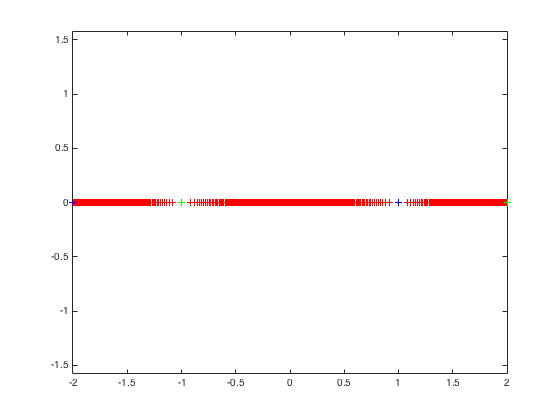
\includegraphics[scale=.5]{one}

\end{frame}



\begin{frame}

$p(z)=\frac{z^4}{4} - \frac{z^3}{3} - \frac{z^2}{2} + z$

\end{frame}


\begin{frame}

$p(z)=\frac{z^4}{4} - \frac{z^3}{3} - \frac{z^2}{2} + z$

\vspace{5mm}

$p'(z)=(z-1)^2(z+1)$

\end{frame}


\begin{frame}

$p(z)=\frac{z^4}{4} - \frac{z^3}{3} - \frac{z^2}{2} + z$ (two critical values $5/12, -11/12$)

\vspace{5mm}

$p'(z)=(z-1)^2(z+1)$

\end{frame}


\begin{frame}

$p(z)=\frac{z^4}{4} - \frac{z^3}{3} - \frac{z^2}{2} + z$ (two critical values $5/12, -11/12$)

\vspace{5mm}

$p'(z)=(z-1)^2(z+1)$

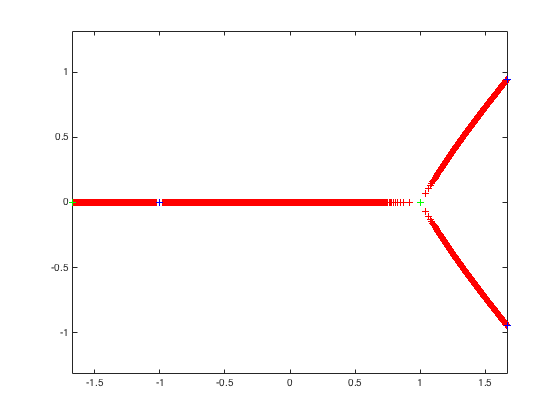
\includegraphics[scale=.5]{two}

\end{frame}








\begin{frame}

{\it Shabat} polynomial - 

\end{frame}


\begin{frame}

{\it Shabat} polynomial - only has two critical values $\pm 1$

\end{frame}



\begin{frame}

{\it Shabat} polynomial - only has two critical values $\pm 1$

\vspace{5mm}

{\bf Proposition:} For any {\it Shabat} polynomial $p(z)$, it is true that $p^{-1}[-1,1]$ is a tree.

\end{frame}




\begin{frame}

{\it Shabat} polynomial - only has two critical values $\pm 1$

\vspace{5mm}

{\bf Proposition:} For any {\it Shabat} polynomial $p(z)$, it is true that $p^{-1}[-1,1]$ is a tree, with $\deg(p)$ edges.

\end{frame}





\begin{frame}

{\it Shabat} polynomial - only has two critical values $\pm 1$

\vspace{5mm}

{\bf Proposition:} For any {\it Shabat} polynomial $p(z)$, it is true that $p^{-1}[-1,1]$ is a tree, with $\deg(p)$ edges.

\vspace{5mm} 

{\bf Theorem {\it (Grothendieck)}:} {\it ALL} combinatorial trees occur as $p^{-1}[-1,1]$ for some {\it Shabat} polynomial $p(z)$.

\vspace{5mm}

\end{frame}




\begin{frame}

{\it Shabat} polynomial - only has two critical values $\pm 1$

\vspace{5mm}

{\bf Proposition:} For any {\it Shabat} polynomial $p(z)$, it is true that $p^{-1}[-1,1]$ is a tree, with $\deg(p)$ edges.

\vspace{5mm} 

{\bf Theorem {\it (Grothendieck)}:} {\it ALL} combinatorial trees occur as $p^{-1}[-1,1]$ for some {\it Shabat} polynomial $p(z)$.

\vspace{5mm}

{\bf Theorem {\it (Bishop)}:} Any {\color{red} continua} can be $\epsilon$-approximated in the {\color{red} Hausdorff metric} by some $p^{-1}[-1,1]$. 

\end{frame}




\begin{frame}

\begin{align*} \text{trees }  \iff \text{ {\it Shabat} polynomials } \end{align*}

\end{frame}


\begin{frame}

\begin{align*} \text{trees }  \iff \text{ {\it Shabat} polynomials } \end{align*}

\vspace{5mm}

\begin{align*} \text{infinite trees }  \iff \text{ {\color{red}Transcendental Functions }} \end{align*}

\end{frame}


\begin{frame}

\begin{align*} \text{trees }  \iff \text{ {\it Shabat} polynomials } \end{align*}

\vspace{5mm}

\begin{align*} \text{infinite trees }  \iff \text{ {\color{red} Subclass of Transcendental Functions } } \end{align*}

\end{frame}


\begin{frame}

\begin{align*} \text{trees }  \iff \text{ {\it Shabat} polynomials } \end{align*}

\vspace{5mm}

\begin{align*} \text{infinite trees }  \iff \text{ {\color{red} Subclass of Transcendental Functions } } \end{align*}

{\color{red} $\mathcal{S}_{2,0}$ } - transcendental functions with two critical values $\pm 1$ and no {\color{red} asymptotic values}

\end{frame}




\begin{frame} 

$\cosh(z) \coloneqq \frac{e^z+e^{-z}}{2}$

\end{frame}


\begin{frame} 

$\cosh(z) \coloneqq \frac{e^z+e^{-z}}{2}$

$\cosh'(z) = \frac{e^z-e^{-z}}{2}$

\end{frame}


\begin{frame} 

$\cosh(z) \coloneqq \frac{e^z+e^{-z}}{2}$

$\cosh'(z) = \frac{e^z-e^{-z}}{2} = 0 \implies z = \pi i \text{n} : n \in \mathbb{Z}$

\end{frame}


\begin{frame} 

$\cosh(z) \coloneqq \frac{e^z+e^{-z}}{2}$

$\cosh'(z) = \frac{e^z-e^{-z}}{2} = 0 \implies z = \pi i \text{n} : n \in \mathbb{Z}$ (critical points)

\end{frame}




\begin{frame} 

$\cosh(z) \coloneqq \frac{e^z+e^{-z}}{2}$

$\cosh'(z) = \frac{e^z-e^{-z}}{2} = 0 \implies z = \pi i \text{n} : n \in \mathbb{Z}$ (critical points)

\vspace{5mm}

critical values: $\pm 1$ 

\end{frame}






\begin{frame}

$T$ - unbounded, locally finite tree

\end{frame}


\begin{frame}

$T$ - unbounded, locally finite tree, with a bipartite labeling of vertices.

\end{frame}


\begin{frame}

$T$ - unbounded, locally finite tree, with a bipartite labeling of vertices.

$\Omega_j$ - components of $\mathbb{C}-T$

\end{frame}



\begin{frame}

$T$ - unbounded, locally finite tree, with a bipartite labeling of vertices.

$\Omega_j$ - components of $\mathbb{C}-T$

$\tau: \cup \Omega_j \rightarrow \mathbb{C}$ - the map conformal on each $\Omega_j$ to $\mathbb{H}_r$

\end{frame}




\begin{frame}

$T$ - unbounded, locally finite tree, with a bipartite labeling of vertices.

$\Omega_j$ - components of $\mathbb{C}-T$

$\tau: \cup \Omega_j \rightarrow \mathbb{C}$ - the map conformal on each $\Omega_j$ to $\mathbb{H}_r$

$V$ - the vertices of $T$. 

\end{frame}





\begin{frame}

$T$ - unbounded, locally finite tree, with a bipartite labeling of vertices.

$\Omega_j$ - components of $\mathbb{C}-T$.

$\tau: \cup \Omega_j \rightarrow \mathbb{C}$ - the map conformal on each $\Omega_j$ to $\mathbb{H}_r$.

$V$ - the vertices of $T$. 

$V_j$ - the image of $V$ under $\tau$ restricted to $\Omega_j$.

\end{frame}



\begin{frame}

$T$ - unbounded, locally finite tree, with a bipartite labeling of vertices.

$\Omega_j$ - components of $\mathbb{C}-T$.

$\tau: \cup \Omega_j \rightarrow \mathbb{C}$ - the map conformal on each $\Omega_j$ to $\mathbb{H}_r$.

$V$ - the vertices of $T$. 

$V_j$ - the image of $V$ under $\tau$ restricted to $\Omega_j$.

For $r > 0$, define $T(r) = \cup_{e\in T} \{z : \textrm{dist}(z,e) < r\textrm{diam}(e) \}$

\end{frame}





\begin{frame}

$T$ - unbounded, locally finite tree, with a bipartite labeling of vertices.

$\Omega_j$ - components of $\mathbb{C}-T$.

$\tau: \cup \Omega_j \rightarrow \mathbb{C}$ - the map conformal on each $\Omega_j$ to $\mathbb{H}_r$.

$V$ - the vertices of $T$. 

$V_j$ - the image of $V$ under $\tau$ restricted to $\Omega_j$.

For $r > 0$, define $T(r) = \cup_{e\in T} \{z : \textrm{dist}(z,e) < r\textrm{diam}(e) \}$

The {\color{red} $\tau$-size} of edge $e$ is the minimum length of the two images $\tau(e)$

\end{frame}




\begin{frame}

$T$ - unbounded, locally finite tree, with a bipartite labeling of vertices.

$\Omega_j$ - components of $\mathbb{C}-T$.

$\tau: \cup \Omega_j \rightarrow \mathbb{C}$ - the map conformal on each $\Omega_j$ to $\mathbb{H}_r$.

$V$ - the vertices of $T$. 

$V_j$ - the image of $V$ under $\tau$ restricted to $\Omega_j$.

For $r > 0$, define $T(r) = \cup_{e\in T} \{z : \textrm{dist}(z,e) < r\textrm{diam}(e) \}$

The $\tau$-size of edge $e$ is the minimum length of the two images $\tau(e)$

\vspace{5mm}

$T$ has uniformly bounded geometry if: 


\end{frame}







\begin{frame}

$T$ - unbounded, locally finite tree, with a bipartite labeling of vertices.

$\Omega_j$ - components of $\mathbb{C}-T$.

$\tau: \cup \Omega_j \rightarrow \mathbb{C}$ - the map conformal on each $\Omega_j$ to $\mathbb{H}_r$.

$V$ - the vertices of $T$. 

$V_j$ - the image of $V$ under $\tau$ restricted to $\Omega_j$.

For $r > 0$, define $T(r) = \cup_{e\in T} \{z : \textrm{dist}(z,e) < r\textrm{diam}(e) \}$

The $\tau$-size of edge $e$ is the minimum length of the two images $\tau(e)$

\vspace{5mm}

$T$ has uniformly bounded geometry if: 

\hspace{5mm} (1) The edges of $T$ are $C^2$ with uniform bounds. 

\end{frame}





\begin{frame}

$T$ - unbounded, locally finite tree, with a bipartite labeling of vertices.

$\Omega_j$ - components of $\mathbb{C}-T$.

$\tau: \cup \Omega_j \rightarrow \mathbb{C}$ - the map conformal on each $\Omega_j$ to $\mathbb{H}_r$.

$V$ - the vertices of $T$. 

$V_j$ - the image of $V$ under $\tau$ restricted to $\Omega_j$.

For $r > 0$, define $T(r) = \cup_{e\in T} \{z : \textrm{dist}(z,e) < r\textrm{diam}(e) \}$

The $\tau$-size of edge $e$ is the minimum length of the two images $\tau(e)$

\vspace{5mm}

$T$ has uniformly bounded geometry if: 

\hspace{5mm} (1) The edges of $T$ are $C^2$ with uniform bounds. 

\hspace{5mm} (2) The angles between adjacent edges are bounded uniformly from zero

\end{frame}






\begin{frame}

$T$ - unbounded, locally finite tree, with a bipartite labeling of vertices.

$\Omega_j$ - components of $\mathbb{C}-T$.

$\tau: \cup \Omega_j \rightarrow \mathbb{C}$ - the map conformal on each $\Omega_j$ to $\mathbb{H}_r$.

$V$ - the vertices of $T$. 

$V_j$ - the image of $V$ under $\tau$ restricted to $\Omega_j$.

For $r > 0$, define $T(r) = \cup_{e\in T} \{z : \textrm{dist}(z,e) < r\textrm{diam}(e) \}$

The $\tau$-size of edge $e$ is the minimum length of the two images $\tau(e)$

\vspace{5mm}

$T$ has uniformly bounded geometry if: 

\hspace{5mm} (1) The edges of $T$ are $C^2$ with uniform bounds. 

\hspace{5mm} (2) The angles between adjacent edges are bounded uniformly from zero

\hspace{5mm} (3) Adjacent edges have uniformly comparable lengths

\end{frame}







\begin{frame}

$T$ - unbounded, locally finite tree, with a bipartite labeling of vertices.

$\Omega_j$ - components of $\mathbb{C}-T$.

$\tau: \cup \Omega_j \rightarrow \mathbb{C}$ - the map conformal on each $\Omega_j$ to $\mathbb{H}_r$.

$V$ - the vertices of $T$. 

$V_j$ - the image of $V$ under $\tau$ restricted to $\Omega_j$.

For $r > 0$, define $T(r) = \cup_{e\in T} \{z : \textrm{dist}(z,e) < r\textrm{diam}(e) \}$

The $\tau$-size of edge $e$ is the minimum length of the two images $\tau(e)$

\vspace{5mm}

$T$ has uniformly bounded geometry if: 

\hspace{5mm} (1) The edges of $T$ are $C^2$ with uniform bounds. 

\hspace{5mm} (2) The angles between adjacent edges are bounded uniformly from zero

\hspace{5mm} (3) Adjacent edges have uniformly comparable lengths

\hspace{5mm} (4) For non-adjacent edges $e, f$, we have $diam(e)/dist(e,f)$ uniformly bounded.

\end{frame}






\begin{frame}

{\tiny $T$ - unbounded, locally finite tree, with a bipartite labeling of vertices.

$\Omega_j$ - components of $\mathbb{C}-T$.

$\tau: \cup \Omega_j \rightarrow \mathbb{C}$ - the map conformal on each $\Omega_j$ to $\mathbb{H}_r$.

$V$ - the vertices of $T$. 

$V_j$ - the image of $V$ under $\tau$ restricted to $\Omega_j$.

For $r > 0$, define $T(r) = \cup_{e\in T} \{z : \textrm{dist}(z,e) < r\textrm{diam}(e) \}$

The $\tau$-size of edge $e$ is the minimum length of the two images $\tau(e)$

\vspace{2.5mm}

$T$ has uniformly bounded geometry if: 

\hspace{5mm} (1) The edges of $T$ are $C^2$ with uniform bounds. 

\hspace{5mm} (2) The angles between adjacent edges are bounded uniformly from zero

\hspace{5mm} (3) Adjacent edges have uniformly comparable lengths

\hspace{5mm} (4) For non-adjacent edges $e, f$, we have $diam(e)/dist(e,f)$ uniformly bounded. 

 }

\vspace{5mm}

{\bf Theorem:} {\it    }  

\end{frame}




\begin{frame}

{\tiny $T$ - unbounded, locally finite tree, with a bipartite labeling of vertices.

$\Omega_j$ - components of $\mathbb{C}-T$.

$\tau: \cup \Omega_j \rightarrow \mathbb{C}$ - the map conformal on each $\Omega_j$ to $\mathbb{H}_r$.

$V$ - the vertices of $T$. 

$V_j$ - the image of $V$ under $\tau$ restricted to $\Omega_j$.

For $r > 0$, define $T(r) = \cup_{e\in T} \{z : \textrm{dist}(z,e) < r\textrm{diam}(e) \}$

The $\tau$-size of edge $e$ is the minimum length of the two images $\tau(e)$

\vspace{2.5mm}

$T$ has uniformly bounded geometry if: 

\hspace{5mm} (1) The edges of $T$ are $C^2$ with uniform bounds. 

\hspace{5mm} (2) The angles between adjacent edges are bounded uniformly from zero

\hspace{5mm} (3) Adjacent edges have uniformly comparable lengths

\hspace{5mm} (4) For non-adjacent edges $e, f$, we have $diam(e)/dist(e,f)$ uniformly bounded. 

 }

\vspace{5mm}

{\bf Theorem:} {\it  Suppose $T$ has bounded geometry  }  

\end{frame}








\begin{frame}

{\tiny $T$ - unbounded, locally finite tree, with a bipartite labeling of vertices.

$\Omega_j$ - components of $\mathbb{C}-T$.

$\tau: \cup \Omega_j \rightarrow \mathbb{C}$ - the map conformal on each $\Omega_j$ to $\mathbb{H}_r$.

$V$ - the vertices of $T$. 

$V_j$ - the image of $V$ under $\tau$ restricted to $\Omega_j$.

For $r > 0$, define $T(r) = \cup_{e\in T} \{z : \textrm{dist}(z,e) < r\textrm{diam}(e) \}$

The $\tau$-size of edge $e$ is the minimum length of the two images $\tau(e)$

\vspace{2.5mm}

$T$ has uniformly bounded geometry if: 

\hspace{5mm} (1) The edges of $T$ are $C^2$ with uniform bounds. 

\hspace{5mm} (2) The angles between adjacent edges are bounded uniformly from zero

\hspace{5mm} (3) Adjacent edges have uniformly comparable lengths

\hspace{5mm} (4) For non-adjacent edges $e, f$, we have $diam(e)/dist(e,f)$ uniformly bounded. 

 }
\vspace{5mm}
{\bf Theorem:} {\it  Suppose $T$ has bounded geometry and every edge has $\tau$-size $\geq \pi.$  }  

\end{frame}





\begin{frame}

{\tiny $T$ - unbounded, locally finite tree, with a bipartite labeling of vertices.

$\Omega_j$ - components of $\mathbb{C}-T$.

$\tau: \cup \Omega_j \rightarrow \mathbb{C}$ - the map conformal on each $\Omega_j$ to $\mathbb{H}_r$.

$V$ - the vertices of $T$. 

$V_j$ - the image of $V$ under $\tau$ restricted to $\Omega_j$.

For $r > 0$, define $T(r) = \cup_{e\in T} \{z : \textrm{dist}(z,e) < r\textrm{diam}(e) \}$

The $\tau$-size of edge $e$ is the minimum length of the two images $\tau(e)$

\vspace{2.5mm}

$T$ has uniformly bounded geometry if: 

\hspace{5mm} (1) The edges of $T$ are $C^2$ with uniform bounds. 

\hspace{5mm} (2) The angles between adjacent edges are bounded uniformly from zero

\hspace{5mm} (3) Adjacent edges have uniformly comparable lengths

\hspace{5mm} (4) For non-adjacent edges $e, f$, we have $diam(e)/dist(e,f)$ uniformly bounded. 

 }
\vspace{5mm}
{\bf Theorem:} {\it  Suppose $T$ has bounded geometry and every edge has $\tau$-size $\geq \pi.$  Then there is an $r_0 > 0$, an entire $f$, and a $K$-quasiconformal $\phi$}  

\end{frame}


\begin{frame}

{\tiny $T$ - unbounded, locally finite tree, with a bipartite labeling of vertices.

$\Omega_j$ - components of $\mathbb{C}-T$.

$\tau: \cup \Omega_j \rightarrow \mathbb{C}$ - the map conformal on each $\Omega_j$ to $\mathbb{H}_r$.

$V$ - the vertices of $T$. 

$V_j$ - the image of $V$ under $\tau$ restricted to $\Omega_j$.

For $r > 0$, define $T(r) = \cup_{e\in T} \{z : \textrm{dist}(z,e) < r\textrm{diam}(e) \}$

The $\tau$-size of edge $e$ is the minimum length of the two images $\tau(e)$

\vspace{2.5mm}

$T$ has uniformly bounded geometry if: 

\hspace{5mm} (1) The edges of $T$ are $C^2$ with uniform bounds. 

\hspace{5mm} (2) The angles between adjacent edges are bounded uniformly from zero

\hspace{5mm} (3) Adjacent edges have uniformly comparable lengths

\hspace{5mm} (4) For non-adjacent edges $e, f$, we have $diam(e)/dist(e,f)$ uniformly bounded. 

 }
\vspace{5mm}
{\bf Theorem:} {\it  Suppose $T$ has bounded geometry and every edge has $\tau$-size $\geq \pi$.  Then there is an $r_0 > 0$, an entire $f$, and a $K$-quasiconformal $\phi$ so that $f \circ \phi = \cosh \circ \tau$ off $T(r_0)$. }  

\end{frame}







\begin{frame}

{\tiny $T$ - unbounded, locally finite tree, with a bipartite labeling of vertices.

$\Omega_j$ - components of $\mathbb{C}-T$.

$\tau: \cup \Omega_j \rightarrow \mathbb{C}$ - the map conformal on each $\Omega_j$ to $\mathbb{H}_r$.

$V$ - the vertices of $T$. 

$V_j$ - the image of $V$ under $\tau$ restricted to $\Omega_j$.

For $r > 0$, define $T(r) = \cup_{e\in T} \{z : \textrm{dist}(z,e) < r\textrm{diam}(e) \}$

The $\tau$-size of edge $e$ is the minimum length of the two images $\tau(e)$

\vspace{2.5mm}

$T$ has uniformly bounded geometry if: 

\hspace{5mm} (1) The edges of $T$ are $C^2$ with uniform bounds. 

\hspace{5mm} (2) The angles between adjacent edges are bounded uniformly from zero

\hspace{5mm} (3) Adjacent edges have uniformly comparable lengths

\hspace{5mm} (4) For non-adjacent edges $e, f$, we have $diam(e)/dist(e,f)$ uniformly bounded. 

 }
\vspace{5mm}
{\bf Theorem:} {\it  Suppose $T$ has bounded geometry and every edge has $\tau$-size $\geq \pi$.  Then there is an $r_0 > 0$, an entire $f$, and a $K$-quasiconformal $\phi$ so that $f \circ \phi = \cosh \circ \tau$ off $T(r_0)$. $K$ depends only on the bounded geometry constants of $T$. }  

\end{frame}







\begin{frame}

{\tiny $T$ - unbounded, locally finite tree, with a bipartite labeling of vertices.

$\Omega_j$ - components of $\mathbb{C}-T$.

$\tau: \cup \Omega_j \rightarrow \mathbb{C}$ - the map conformal on each $\Omega_j$ to $\mathbb{H}_r$.

$V$ - the vertices of $T$. 

$V_j$ - the image of $V$ under $\tau$ restricted to $\Omega_j$.

For $r > 0$, define $T(r) = \cup_{e\in T} \{z : \textrm{dist}(z,e) < r\textrm{diam}(e) \}$

The $\tau$-size of edge $e$ is the minimum length of the two images $\tau(e)$

\vspace{2.5mm}

$T$ has uniformly bounded geometry if: 

\hspace{5mm} (1) The edges of $T$ are $C^2$ with uniform bounds. 

\hspace{5mm} (2) The angles between adjacent edges are bounded uniformly from zero

\hspace{5mm} (3) Adjacent edges have uniformly comparable lengths

\hspace{5mm} (4) For non-adjacent edges $e, f$, we have $diam(e)/dist(e,f)$ uniformly bounded. 

 }
\vspace{5mm}
{\bf Theorem:} {\it  Suppose $T$ has bounded geometry and every edge has $\tau$-size $\geq \pi$.  Then there is an $r_0 > 0$, an entire $f$, and a $K$-quasiconformal $\phi$ so that $f \circ \phi = \cosh \circ \tau$ off $T(r_0)$. $K$ depends only on the bounded geometry constants of $T$. The only critical values of $f$ are $\pm 1$ and f has no asymptotic values.}  

\end{frame}

%----------------------------------------------------------------------------------------






\begin{frame}

$f: \mathbb{C} \rightarrow \mathbb{C}$ entire function

\end{frame}



\begin{frame}

$f: \mathbb{C} \rightarrow \mathbb{C}$ entire function

\vspace{2.5mm}


$f^{\circ n}$ is normal in an open set $U$ 

\end{frame}



\begin{frame}

$f: \mathbb{C} \rightarrow \mathbb{C}$ entire function

\vspace{2.5mm}

$f^{\circ n}$ is normal in an open set $U$ if every sequence of $f^{\circ k}$ contains a further subsequence converging locally uniformly to a holomorphic function $g: U \rightarrow \overline{\mathbb{C}}$

\end{frame}





\begin{frame}

$f: \mathbb{C} \rightarrow \mathbb{C}$ entire function

\vspace{2.5mm}

$f^{\circ n}$ is normal in an open set $U$ if every sequence of $f^{\circ k}$ contains a further subsequence converging locally uniformly to a holomorphic function $g: U \rightarrow \overline{\mathbb{C}}$

\vspace{2.5mm}

The Fatou set of $f$ is the set of points $z \in \mathbb{C}$ for which $f$ is normal in some neighborhood of $z$.

\end{frame}



\begin{frame}

$f: \mathbb{C} \rightarrow \mathbb{C}$ entire function

\vspace{2.5mm}

$f^{\circ n}$ is normal in an open set $U$ if every sequence of $f^{\circ k}$ contains a further subsequence converging locally uniformly to a holomorphic function $g: U \rightarrow \overline{\mathbb{C}}$

\vspace{2.5mm}

The Fatou set of $f$ is the set of points $z \in \mathbb{C}$ for which $f$ is normal in some neighborhood of $z$. The components of the Fatou set are called Fatou components.

\end{frame}






\begin{frame}

$f: \mathbb{C} \rightarrow \mathbb{C}$ entire function

\vspace{2.5mm}

$f^{\circ n}$ is normal in an open set $U$ if every sequence of $f^{\circ k}$ contains a further subsequence converging locally uniformly to a holomorphic function $g: U \rightarrow \overline{\mathbb{C}}$

\vspace{2.5mm}

The Fatou set of $f$ is the set of points $z \in \mathbb{C}$ for which $f$ is normal in some neighborhood of $z$. The components of the Fatou set are called Fatou components.

\vspace{2.5mm} 

A Fatou component $U$ is called {\it wandering} if $f^n(U) \cap f^m(U) = \emptyset$ for all $n,m \in \mathbb{N}, n \not = m$

\end{frame}





\begin{frame}

{\bf Theorem:} {\it (Sullivan) Rational maps don't have wandering domains.}

\end{frame}


\begin{frame}

{\bf Theorem:} {\it (Sullivan) Rational maps don't have wandering domains.}

\vspace{2.5mm} 

For $f: \mathbb{C} \rightarrow \mathbb{C}$, the singular set $S(f)$ consists of the critical values and asymptotic values of $f$.

\vspace{2.5mm}

\end{frame}


\begin{frame}

{\bf Theorem:} {\it (Sullivan) Rational maps don't have wandering domains.}

\vspace{2.5mm} 

For $f: \mathbb{C} \rightarrow \mathbb{C}$, the singular set $S(f)$ consists of the critical values and asymptotic values of $f$.

\vspace{2.5mm}

The {\it Speiser} class $\mathcal{S}$ consists of those transcendental functions for which $S(f)$ is finite. 

\end{frame}






\begin{frame}

{\bf Theorem:} {\it (Sullivan) Rational maps don't have wandering domains.}

\vspace{2.5mm} 

For $f: \mathbb{C} \rightarrow \mathbb{C}$, the singular set $S(f)$ consists of the critical values and asymptotic values of $f$.

\vspace{2.5mm}

The {\it Speiser} class $\mathcal{S}$ consists of those transcendental functions for which $S(f)$ is finite. 

\vspace{2.5mm} 

{\bf Theorem:} {\it (Golberg and Keen, Eremenko and Lyubich)  Functions in the Speiser Class don't have wandering domains.}

\end{frame}






\begin{frame}

{\bf Theorem:} {\it (Sullivan) Rational maps don't have wandering domains.}

\vspace{2.5mm} 

For $f: \mathbb{C} \rightarrow \mathbb{C}$, the singular set $S(f)$ consists of the critical values and asymptotic values of $f$.

\vspace{2.5mm}

The {\it Speiser} class $\mathcal{S}$ consists of those transcendental functions for which $S(f)$ is finite. 

\vspace{2.5mm} 

{\bf Theorem:} {\it (Golberg and Keen, Eremenko and Lyubich)  Functions in the Speiser Class don't have wandering domains.}

\vspace{2.5mm}

The Eremenko-Lyubich class $\mathcal{B}$ consists of those transcendental functions with bounded singular set. 

\end{frame}














\begin{frame} 

$S^+ = \{ x + iy : x > 0, |y| < \pi/2 \}$ 

\end{frame}





\begin{frame} 

$S^+ = \{ x + iy : x > 0, |y| < \pi/2 \}$ is mapped conformally to $\mathbb{H}_r$ by $\lambda\cdot\sinh$.  

\end{frame}



\begin{frame} 

$S^+ = \{ x + iy : x > 0, |y| < \pi/2 \}$ is mapped conformally to $\mathbb{H}_r$ by $\lambda\cdot\sinh$. Then holomorphically to $\mathbb{C} - [-1,1]$ by $\cosh$.

\end{frame}




\begin{frame} 

$S^+ = \{ x + iy : x > 0, |y| < \pi/2 \}$ is mapped conformally to $\mathbb{H}_r$ by $\lambda\cdot\sinh$. Then holomorphically to $\mathbb{C} - [-1,1]$ by $\cosh$.

\vspace{2.5mm}

$a_n = \cosh^{-1}\left( \frac{\pi}{\lambda} \left \lfloor{ \frac{\lambda}{\pi} \cosh(n\pi) }\right \rfloor \right)$

\end{frame}





\begin{frame} 

$S^+ = \{ x + iy : x > 0, |y| < \pi/2 \}$ is mapped conformally to $\mathbb{H}_r$ by $\lambda\cdot\sinh$. Then holomorphically to $\mathbb{C} - [-1,1]$ by $\cosh$.

\vspace{2.5mm}

$a_n = \cosh^{-1}\left( \frac{\pi}{\lambda} \left \lfloor{ \frac{\lambda}{\pi} \cosh(n\pi) }\right \rfloor \right)$

\vspace{2.5mm}

$z_n = a_n + i\pi$

\end{frame}




\begin{frame} 

$S^+ = \{ x + iy : x > 0, |y| < \pi/2 \}$ is mapped conformally to $\mathbb{H}_r$ by $\lambda\cdot\sinh$. Then holomorphically to $\mathbb{C} - [-1,1]$ by $\cosh$.

\vspace{2.5mm}

$a_n = \cosh^{-1}\left( \frac{\pi}{\lambda} \left \lfloor{ \frac{\lambda}{\pi} \cosh(n\pi) }\right \rfloor \right)$

\vspace{2.5mm}

$z_n = a_n + i\pi, D_n = \{ z \in \mathbb{C} : \left| z - z_n \right| < 1\} $

\end{frame}



\begin{frame} 

$S^+ = \{ x + iy : x > 0, |y| < \pi/2 \}$ is mapped conformally to $\mathbb{H}_r$ by $\lambda\cdot\sinh$. Then holomorphically to $\mathbb{C} - [-1,1]$ by $\cosh$.

\vspace{2.5mm}

$a_n = \cosh^{-1}\left( \frac{\pi}{\lambda} \left \lfloor{ \frac{\lambda}{\pi} \cosh(n\pi) }\right \rfloor \right)$

\vspace{2.5mm}

$z_n = a_n + i\pi, D_n = \{ z \in \mathbb{C} : \left| z - z_n \right| < 1\} $ is mapped holomorphically to $|z|<1$ by $z\rightarrow (z - z_n)^{d_n}$.

\end{frame}






\begin{frame} 

$S^+ = \{ x + iy : x > 0, |y| < \pi/2 \}$ is mapped conformally to $\mathbb{H}_r$ by $\lambda\cdot\sinh$. Then holomorphically to $\mathbb{C} - [-1,1]$ by $\cosh$.

\vspace{2.5mm}

$a_n = \cosh^{-1}\left( \frac{\pi}{\lambda} \left \lfloor{ \frac{\lambda}{\pi} \cosh(n\pi) }\right \rfloor \right)$

\vspace{2.5mm}

$z_n = a_n + i\pi, D_n = \{ z \in \mathbb{C} : \left| z - z_n \right| < 1\} $ is mapped holomorphically to $|z|<1$ by $z\rightarrow (z - z_n)^{d_n}$. Then by a quasiconformal map $\rho$ of the disc so that: 

\end{frame}





\begin{frame} 

$S^+ = \{ x + iy : x > 0, |y| < \pi/2 \}$ is mapped conformally to $\mathbb{H}_r$ by $\lambda\cdot\sinh$. Then holomorphically to $\mathbb{C} - [-1,1]$ by $\cosh$.

\vspace{2.5mm}

$a_n = \cosh^{-1}\left( \frac{\pi}{\lambda} \left \lfloor{ \frac{\lambda}{\pi} \cosh(n\pi) }\right \rfloor \right)$

\vspace{2.5mm}

$z_n = a_n + i\pi, D_n = \{ z \in \mathbb{C} : \left| z - z_n \right| < 1\} $ is mapped holomorphically to $|z|<1$ by $z\rightarrow (z - z_n)^{d_n}$. Then by a quasiconformal map $\rho_n$ of the disc so that: 

\hspace{5mm} (1) $\rho_n(z)=z$ for $z\in\partial\mathbb{D}$

\end{frame}





\begin{frame} 

$S^+ = \{ x + iy : x > 0, |y| < \pi/2 \}$ is mapped conformally to $\mathbb{H}_r$ by $\lambda\cdot\sinh$. Then holomorphically to $\mathbb{C} - [-1,1]$ by $\cosh$.

\vspace{2.5mm}

$a_n = \cosh^{-1}\left( \frac{\pi}{\lambda} \left \lfloor{ \frac{\lambda}{\pi} \cosh(n\pi) }\right \rfloor \right)$

\vspace{2.5mm}

$z_n = a_n + i\pi, D_n = \{ z \in \mathbb{C} : \left| z - z_n \right| < 1\} $ is mapped holomorphically to $|z|<1$ by $z\rightarrow (z - z_n)^{d_n}$. Then by a quasiconformal map $\rho_n$ of the disc so that: 

\hspace{5mm} (1) $\rho_n(z)=z$ for $z\in\partial\mathbb{D}$

\hspace{5mm} (2) $\rho_n(0)=w_n$ where $w_n$ is a point near $1/2$.

\end{frame}




\begin{frame} 

$S^+ = \{ x + iy : x > 0, |y| < \pi/2 \}$ is mapped conformally to $\mathbb{H}_r$ by $\lambda\cdot\sinh$. Then holomorphically to $\mathbb{C} - [-1,1]$ by $\cosh$.

\vspace{2.5mm}

$a_n = \cosh^{-1}\left( \frac{\pi}{\lambda} \left \lfloor{ \frac{\lambda}{\pi} \cosh(n\pi) }\right \rfloor \right)$

\vspace{2.5mm}

$z_n = a_n + i\pi, D_n = \{ z \in \mathbb{C} : \left| z - z_n \right| < 1\} $ is mapped holomorphically to $|z|<1$ by $z\rightarrow (z - z_n)^{d_n}$. Then by a quasiconformal map $\rho_n$ of the disc so that: 

\hspace{5mm} (1) $\rho_n(z)=z$ for $z\in\partial\mathbb{D}$

\hspace{5mm} (2) $\rho_n(0)=w_n$ where $w_n$ is a point near $1/2$.

\hspace{5mm} (3) $\rho_n$ is conformal on $\frac{3}{4}\mathbb{D}$

\end{frame}




\begin{frame} 

$S^+ = \{ x + iy : x > 0, |y| < \pi/2 \}$ is mapped conformally to $\mathbb{H}_r$ by $\lambda\cdot\sinh$. Then holomorphically to $\mathbb{C} - [-1,1]$ by $\cosh$.

\vspace{2.5mm}

$a_n = \cosh^{-1}\left( \frac{\pi}{\lambda} \left \lfloor{ \frac{\lambda}{\pi} \cosh(n\pi) }\right \rfloor \right)$

\vspace{2.5mm}

$z_n = a_n + i\pi, D_n = \{ z \in \mathbb{C} : \left| z - z_n \right| < 1\} $ is mapped holomorphically to $|z|<1$ by $z\rightarrow (z - z_n)^{d_n}$. Then by a quasiconformal map $\rho_n$ of the disc so that: 

\hspace{5mm} (1) $\rho_n(z)=z$ for $z\in\partial\mathbb{D}$

\hspace{5mm} (2) $\rho_n(0)=w_n$ where $w_n$ is a point near $1/2$.

\hspace{5mm} (3) $\rho_n$ is conformal on $\frac{3}{4}\mathbb{D}$

\hspace{5mm} (4) $\rho_n$ is quasiconformal on $\mathbb{D}$. 

\end{frame}





\begin{frame} 

{\tiny $S^+ = \{ x + iy : x > 0, |y| < \pi/2 \}$ is mapped conformally to $\mathbb{H}_r$ by $\lambda\cdot\sinh$. Then holomorphically to $\mathbb{C} - [-1,1]$ by $\cosh$.

\vspace{2.5mm}

$a_n = \cosh^{-1}\left( \frac{\pi}{\lambda} \left \lfloor{ \frac{\lambda}{\pi} \cosh(n\pi) }\right \rfloor \right)$

\vspace{2.5mm}

$z_n = a_n + i\pi, D_n = \{ z \in \mathbb{C} : \left| z - z_n \right| < 1\} $ is mapped holomorphically to $|z|<1$ by $z\rightarrow (z - z_n)^{d_n}$. Then by a quasiconformal map $\rho_n$ of the disc so that: 

\hspace{5mm} (1) $\rho_n(z)=z$ for $z\in\partial\mathbb{D}$

\hspace{5mm} (2) $\rho_n(0)=w_n$ where $w_n$ is a point near $1/2$.

\hspace{5mm} (3) $\rho_n$ is conformal on $\frac{3}{4}\mathbb{D}$

\hspace{5mm} (4) $\rho_n$ is quasiconformal on $\mathbb{D}$.  

}

\vspace{5mm}

{\bf Theorem:} 


\end{frame}






\begin{frame} 

{\tiny $S^+ = \{ x + iy : x > 0, |y| < \pi/2 \}$ is mapped conformally to $\mathbb{H}_r$ by $\lambda\cdot\sinh$. Then holomorphically to $\mathbb{C} - [-1,1]$ by $\cosh$.

\vspace{2.5mm}

$a_n = \cosh^{-1}\left( \frac{\pi}{\lambda} \left \lfloor{ \frac{\lambda}{\pi} \cosh(n\pi) }\right \rfloor \right)$

\vspace{2.5mm}

$z_n = a_n + i\pi, D_n = \{ z \in \mathbb{C} : \left| z - z_n \right| < 1\} $ is mapped holomorphically to $|z|<1$ by $z\rightarrow (z - z_n)^{d_n}$. Then by a quasiconformal map $\rho_n$ of the disc so that: 

\hspace{5mm} (1) $\rho_n(z)=z$ for $z\in\partial\mathbb{D}$

\hspace{5mm} (2) $\rho_n(0)=w_n$ where $w_n$ is a point near $1/2$.

\hspace{5mm} (3) $\rho_n$ is conformal on $\frac{3}{4}\mathbb{D}$

\hspace{5mm} (4) $\rho_n$ is quasiconformal on $\mathbb{D}$.  

}

\vspace{5mm}

{\bf Theorem:}  {\it For every choice of parameters $\lambda, (d_n), (w_n)$ with $\lambda \in \pi\mathbb{N}, d_n \in 2\mathbb{N}$}


\end{frame}









\begin{frame} 

{\tiny $S^+ = \{ x + iy : x > 0, |y| < \pi/2 \}$ is mapped conformally to $\mathbb{H}_r$ by $\lambda\cdot\sinh$. Then holomorphically to $\mathbb{C} - [-1,1]$ by $\cosh$.

\vspace{2.5mm}

$a_n = \cosh^{-1}\left( \frac{\pi}{\lambda} \left \lfloor{ \frac{\lambda}{\pi} \cosh(n\pi) }\right \rfloor \right)$

\vspace{2.5mm}

$z_n = a_n + i\pi, D_n = \{ z \in \mathbb{C} : \left| z - z_n \right| < 1\} $ is mapped holomorphically to $|z|<1$ by $z\rightarrow (z - z_n)^{d_n}$. Then by a quasiconformal map $\rho_n$ of the disc so that: 

\hspace{5mm} (1) $\rho_n(z)=z$ for $z\in\partial\mathbb{D}$

\hspace{5mm} (2) $\rho_n(0)=w_n$ where $w_n$ is a point near $1/2$.

\hspace{5mm} (3) $\rho_n$ is conformal on $\frac{3}{4}\mathbb{D}$

\hspace{5mm} (4) $\rho_n$ is quasiconformal on $\mathbb{D}$.  

}

\vspace{5mm}

{\bf Theorem:}  {\it For every choice of parameters $\lambda, (d_n), (w_n)$ with $\lambda \in \pi\mathbb{N}, d_n \in 2\mathbb{N}$, there exists a transcendental $f$ and a quasiconformal $\phi: \mathbb{C}\rightarrow\mathbb{C}$ so that:}


\end{frame}








\begin{frame} 

{\tiny $S^+ = \{ x + iy : x > 0, |y| < \pi/2 \}$ is mapped conformally to $\mathbb{H}_r$ by $\lambda\cdot\sinh$. Then holomorphically to $\mathbb{C} - [-1,1]$ by $\cosh$.

\vspace{1.25mm}

$a_n = \cosh^{-1}\left( \frac{\pi}{\lambda} \left \lfloor{ \frac{\lambda}{\pi} \cosh(n\pi) }\right \rfloor \right)$

\vspace{1.25mm}

$z_n = a_n + i\pi, D_n = \{ z \in \mathbb{C} : \left| z - z_n \right| < 1\} $ is mapped holomorphically to $|z|<1$ by $z\rightarrow (z - z_n)^{d_n}$. Then by a quasiconformal map $\rho_n$ of the disc so that: 

\hspace{5mm} (1) $\rho_n(z)=z$ for $z\in\partial\mathbb{D}$

\hspace{5mm} (2) $\rho_n(0)=w_n$ where $w_n$ is a point near $1/2$.

\hspace{5mm} (3) $\rho_n$ is conformal on $\frac{3}{4}\mathbb{D}$

\hspace{5mm} (4) $\rho_n$ is quasiconformal on $\mathbb{D}$.  

}

\vspace{5mm}

{\bf Theorem:}  {\it For every choice of parameters $\lambda, (d_n), (w_n)$ with $\lambda \in \pi\mathbb{N}, d_n \in 2\mathbb{N}$, there exists a transcendental $f$ and a quasiconformal $\phi: \mathbb{C}\rightarrow\mathbb{C}$ so that:}

\hspace{5mm} (1) $f(\overline{z}) = \overline{f(z)}, f(-z)=f(z)$


\end{frame}







\begin{frame} 

{\tiny $S^+ = \{ x + iy : x > 0, |y| < \pi/2 \}$ is mapped conformally to $\mathbb{H}_r$ by $\lambda\cdot\sinh$. Then holomorphically to $\mathbb{C} - [-1,1]$ by $\cosh$.

\vspace{1.25mm}

$a_n = \cosh^{-1}\left( \frac{\pi}{\lambda} \left \lfloor{ \frac{\lambda}{\pi} \cosh(n\pi) }\right \rfloor \right)$

\vspace{1.25mm}

$z_n = a_n + i\pi, D_n = \{ z \in \mathbb{C} : \left| z - z_n \right| < 1\} $ is mapped holomorphically to $|z|<1$ by $z\rightarrow (z - z_n)^{d_n}$. Then by a quasiconformal map $\rho_n$ of the disc so that: 

\hspace{5mm} (1) $\rho_n(z)=z$ for $z\in\partial\mathbb{D}$

\hspace{5mm} (2) $\rho_n(0)=w_n$ where $w_n$ is a point near $1/2$.

\hspace{5mm} (3) $\rho_n$ is conformal on $\frac{3}{4}\mathbb{D}$

\hspace{5mm} (4) $\rho_n$ is quasiconformal on $\mathbb{D}$.  

}

\vspace{5mm}

{\bf Theorem:}  {\it For every choice of parameters $\lambda, (d_n), (w_n)$ with $\lambda \in \pi\mathbb{N}, d_n \in 2\mathbb{N}$, there exists a transcendental $f$ and a quasiconformal $\phi: \mathbb{C}\rightarrow\mathbb{C}$ so that:}

\hspace{5mm} (1) $f(\overline{z}) = \overline{f(z)}, f(-z)=f(z)$

\hspace{5mm} (2) \[ f(z) = \begin{cases} 
      \cosh(\lambda\sinh(\phi(z))) & \textrm{ if } \phi(z)\in S^+ \\
      \rho_n((\phi(z)-z_n)^{d_n}) & \textrm{ if } \phi(z)\in D_n \\
   \end{cases} \]

\end{frame}








\begin{frame} 

{\tiny $S^+ = \{ x + iy : x > 0, |y| < \pi/2 \}$ is mapped conformally to $\mathbb{H}_r$ by $\lambda\cdot\sinh$. Then holomorphically to $\mathbb{C} - [-1,1]$ by $\cosh$.

\vspace{1.25mm}

$a_n = \cosh^{-1}\left( \frac{\pi}{\lambda} \left \lfloor{ \frac{\lambda}{\pi} \cosh(n\pi) }\right \rfloor \right)$

\vspace{1.25mm}

$z_n = a_n + i\pi, D_n = \{ z \in \mathbb{C} : \left| z - z_n \right| < 1\} $ is mapped holomorphically to $|z|<1$ by $z\rightarrow (z - z_n)^{d_n}$. Then by a quasiconformal map $\rho_n$ of the disc so that: 

\hspace{5mm} (1) $\rho_n(z)=z$ for $z\in\partial\mathbb{D}$

\hspace{5mm} (2) $\rho_n(0)=w_n$ where $w_n$ is a point near $1/2$.

\hspace{5mm} (3) $\rho_n$ is conformal on $\frac{3}{4}\mathbb{D}$

\hspace{5mm} (4) $\rho_n$ is quasiconformal on $\mathbb{D}$.  

}

\vspace{5mm}

{\bf Theorem:}  {\it For every choice of parameters $\lambda, (d_n), (w_n)$ with $\lambda \in \pi\mathbb{N}, d_n \in 2\mathbb{N}$, there exists a transcendental $f$ and a quasiconformal $\phi: \mathbb{C}\rightarrow\mathbb{C}$ so that:}

\hspace{5mm} (1) $f(\overline{z}) = \overline{f(z)}, f(-z)=f(z)$

\hspace{5mm} (2) \[ f(z) = \begin{cases} 
      \cosh(\lambda\sinh(\phi(z))) & \textrm{ if } \phi(z)\in S^+ \\
      \rho_n((\phi(z)-z_n)^{d_n}) & \textrm{ if } \phi(z)\in D_n \\
   \end{cases} \]
   
\hspace{5mm} (3) $f$ has no asymptotic values and its set of critical values is $\pm1$ and $\overline{\{w_n: n \geq 1\}}$

\end{frame}









\begin{frame} 

{\tiny $S^+ = \{ x + iy : x > 0, |y| < \pi/2 \}$ is mapped conformally to $\mathbb{H}_r$ by $\lambda\cdot\sinh$. Then holomorphically to $\mathbb{C} - [-1,1]$ by $\cosh$.

\vspace{1.25mm}

$a_n = \cosh^{-1}\left( \frac{\pi}{\lambda} \left \lfloor{ \frac{\lambda}{\pi} \cosh(n\pi) }\right \rfloor \right)$

\vspace{1.25mm}

$z_n = a_n + i\pi, D_n = \{ z \in \mathbb{C} : \left| z - z_n \right| < 1\} $ is mapped holomorphically to $|z|<1$ by $z\rightarrow (z - z_n)^{d_n}$. Then by a quasiconformal map $\rho_n$ of the disc so that: 

\hspace{5mm} (1) $\rho_n(z)=z$ for $z\in\partial\mathbb{D}$

\hspace{5mm} (2) $\rho_n(0)=w_n$ where $w_n$ is a point near $1/2$.

\hspace{5mm} (3) $\rho_n$ is conformal on $\frac{3}{4}\mathbb{D}$

\hspace{5mm} (4) $\rho_n$ is quasiconformal on $\mathbb{D}$.  

}

\vspace{5mm}

{\bf Theorem:}  {\it For every choice of parameters $\lambda, (d_n), (w_n)$ with $\lambda \in \pi\mathbb{N}, d_n \in 2\mathbb{N}$, there exists a transcendental $f$ and a quasiconformal $\phi: \mathbb{C}\rightarrow\mathbb{C}$ so that:}

\hspace{5mm} (1) $f(\overline{z}) = \overline{f(z)}, f(-z)=f(z)$

\hspace{5mm} (2) \[ f(z) = \begin{cases} 
      \cosh(\lambda\sinh(\phi(z))) & \textrm{ if } \phi(z)\in S^+ \\
      \rho_n((\phi(z)-z_n)^{d_n}) & \textrm{ if } \phi(z)\in D_n \\
   \end{cases} \]
   
\hspace{5mm} (3) $f$ has no asymptotic values and its set of critical values is $\pm1$ and $\overline{\{w_n: n \geq 1\}}$

\hspace{5mm} (4) $\phi(0)=0, \phi(\mathbb{R})=\mathbb{R}$ and $\phi$ is conformal in $S^+$.


\end{frame}










%----------------------------------------------------------------------------------------
%----------------------------------------------------------------------------------------







%------------------------------------------------

\begin{frame}
\frametitle{References}
\footnotesize{
\begin{thebibliography}{99} % Beamer does not support BibTeX so references must be inserted manually as below
\bibitem[QCVSDkl]{p1}  Chris Bishop (2014)
\newblock Constructing Entire Functions By Quasiconformal Folding
\newblock \emph{Acta Mathematica}

\bibitem[BRMFCADDkl]{p1} Nuria Fagella, Sebastien Godillion, and Xavier Jarque (2014)
\newblock Wandering domains for composition of entire functions
\newblock \emph{Journal of Mathematical Analysis and Applications} 


\end{thebibliography}
}
\end{frame}

%------------------------------------------------

%----------------------------------------------------------------------------------------

\end{document} 